\documentclass[twoside,twocolumn,11pt]{extarticle}

\usepackage{textcase}
\usepackage{amsthm}
\usepackage{amssymb}
%\newtheorem{thm}{Theorem}
\theoremstyle{definition}
%\newtheorem{defn}[thm]{Definition} % definition numbers are dependent on theorem numbers
%\newtheorem{exmp}[thm]{Example}

\usepackage{blindtext} % Package to generate dummy text throughout this template 

\usepackage[sc]{mathpazo} % Use the Palatino font
\usepackage[T1]{fontenc} % Use 8-bit encoding that has 256 glyphs
\linespread{1.05} % Line spacing - Palatino needs more space between lines
\usepackage{microtype} % Slightly tweak font spacing for aesthetics

\usepackage[italian]{babel} % Language hyphenation and typographical rules
\usepackage[utf8]{inputenc}

\usepackage[hmarginratio=1:1,top=32mm,columnsep=20pt]{geometry} % Document margins
\usepackage[hang,small,labelfont=bf,up,textfont=it,up]{caption} % Custom captions under/above floats in tables or figures
\usepackage{booktabs} % Horizontal rules in tables

\usepackage{graphicx}
\usepackage{float}

\usepackage{lettrine} % The lettrine is the first enlarged letter at the beginning of the text

\usepackage{enumitem} % Customized lists
\setlist[itemize]{noitemsep} % Make itemize lists more compact

\usepackage{abstract} % Allows abstract customization
\renewcommand{\abstractnamefont}{\normalfont\bfseries} % Set the "Abstract" text to bold
\renewcommand{\abstracttextfont}{\normalfont\small\itshape} % Set the abstract itself to small italic text

\usepackage{titlesec} % Allows customization of titles
\renewcommand\thesection{\Roman{section}} % Roman numerals for the sections
\renewcommand\thesubsection{\roman{subsection}} % roman numerals for subsections
\titleformat{\section}[block]{\large\scshape\centering}{\thesection.}{1em}{} % Change the look of the section titles
\titleformat{\subsection}[block]{\large}{\thesubsection.}{1em}{} % Change the look of the section titles

\usepackage{fancyhdr} % Headers and footers
\pagestyle{fancy} % All pages have headers and footers
\fancyhead{} % Blank out the default header
\fancyfoot{} % Blank out the default footer
\fancyhead[C]{Running title $\bullet$ May 2016 $\bullet$ Vol. XXI, No. 1} % Custom header text
\fancyfoot[RO,LE]{\thepage} % Custom footer text

\usepackage{titling} % Customizing the title section

\usepackage{hyperref} % For hyperlinks in the PDF

% Title Section
\setlength{\droptitle}{-4\baselineskip} % Move the title up

\pretitle{\begin{center}\Huge\bfseries} % Article title formatting
\posttitle{\end{center}} % Article title closing formatting
\title{Rilevamento automatico della Prominenza Prosodica nel parlato in Italiano: Reti Neurali Ricorsive} % Article title
\author{%
\textsc{Maxim Gaina} \\[1ex] % Your name
\normalsize Università di Bologna\thanks{Progetto per il corso di Elaborazione del Linguaggio Naturale, A.A. 2016/2017, prof. Fabio Tamburini.} \\ % Your institution
\normalsize \href{mailto:maxim.gaina@studio.unibo.it}{maxim.gaina@studio.unibo.it}
%\and % Uncomment if 2 authors are required, duplicate these 4 lines if more
%\textsc{Jane Smith}\thanks{Corresponding author} \\[1ex] % Second author's name
%\normalsize University of Utah \\ % Second author's institution
%\normalsize \href{mailto:jane@smith.com}{jane@smith.com} % Second author's email address
}
\date{\today} % Leave empty to omit a date
\renewcommand{\maketitlehookd}{%
\begin{abstract}
\noindent Nel parlato, la prominenza prosodica è un fenomeno percettivo che può influire pesantemente sulla semantica delle frasi pronunciate, per questo guadagna un ruolo fondamentale nella comunicazione umana. Sono stati svolti in passato diversi sperimenti per rilevare le sillabe prominenti all'interno di una frase, che prevedevano l'utilizzo di svariati strumenti offerti dall'ambito dell'Apprendimento Automatico o modelli rule-based. L'obiettivo di questo lavoro di progetto è impiegare, per la prima volta nella lingua italiana, le reti neurali ricorsive; valutare successivamente i benefici e infine confrontarli con i metodi precedentemente usati.
\end{abstract}
}

\begin{document}

\maketitle

\tableofcontents

\section*{Introduzione}
	\lettrine[nindent = 0.4em,lines=3]{O}\space\MakeTextLowercase{g}ni lingua possiede un suo insieme di tratti soprasegmentali, che caratterizzano la relativa sequenza lineare del parlato, e i vari rapporti tra foni che compongono tale sequenza. Tali informazioni prosodiche sono spesso cruciali per disambiguare espressioni sintattiche. Per capire, in breve, si prenda l'esempio riportato in \cite{bib:fenomeni-prosodici-prominenza}:
	\begin{itemize}
		\item[a.] \textit{È stato Luigi?}
		\item[b.] \textit{È stato Luigi.}
	\end{itemize}

	In italiano le frasi interrogative sono un esempio di come il profilo intonativo del parlante sia fondamentale, perchè sintatticamente non sono marcate in alcun modo. Nel primo caso si ha un andamento finale ascendente, mentre nella frase dichiarativa tipicamente si tratta di un profilo finale discendente. In altri casi invece, il parlante accentua e/o allunga determinate parole, per concentrare l'attenzione dell'ascoltatore proprio in quel punto della sequenza.	 Si tratta ancora di informazioni difficilmente trasmissibili o per niente trasmissibili per vie sintattiche. I fenomeni prosidici sono quindi l'intonazione, il ritmo, la velocità di elocuzione, le pause e così via. L'oggetto di studio in questo lavoro è la \textbf{prominenza prosodica}, per la quale, più tardi, si cercherà di dare una definizione più esatta. Lo scopo ultimo, è quello di impiegare un particolare tipo di \textit{Reti Neurali Ricorsive} (\texttt{RNN}), cioè le \textit{Long-Short Term Memory} per l'identificazione automatica delle sillabe prominenti. Ancora meglio, si può dire che questo sia un problema di classificazione delle sillabe, prominenti e non, dove le caratteristiche di ogni sillaba dipendono dall'intero contesto in cui si trovano.
	
	Verrà qui esposto il modo in cui è stato affrontato il problema d'esame, preceduto però dalle informazioni necessarie allo studente per capire il problema trattato e il suo contesto, cioè dove si colloca all'interno del \textit{Natural Language Processing}. La relazione avrà quindi la seguente struttura:
	\begin{itemize}
		\item nella prima sezione si cercherà di definire meglio il dominio del problema, restringendolo;
		\item nella seconda sezione verranno spiegati brevemente i principi che stanno alla base delle \texttt{RNN}, e del perché risultano utili;
		\item la terza sezione
	\end{itemize}
	
\section{Prominenza Prosodica}\label{sec:prom}
	È stato detto che si vuole identificare automaticamente la prominenza, ma cosa significa esattamente? Non è proprio immediato dare una definizione, dal momento che gli studiosi addentratisi nel problema, arrivarono spesso a conclusioni divergenti, proponendo teorie e metodi diversi. Esaminando qualche rasségna in merito (\cite[Capitolo 1]{bib:fenomeni-prosodici-prominenza} e \cite{bib:prominence-by-acoustic-analyses}) è possibile vederlo. Talvolta i ricercatori vanno letteralmente in conflitto ridefinendo lo stesso termine, come per esempio lo \textit{stress}. Riprendendo però quanto detto in \cite{bib:prominence-by-acoustic-analyses}, si può così definire la prominenza:
	\theoremstyle{plain}
	\newtheorem{definition}{Definizione}
	\begin{definition}[Prominenza Prosodica]\label{def:prosodic-prominency}
		La prominenza prosodica è un fenomeno percettivo, continuo nella sua natura, che enfatizza alcune unità linguistiche e segmentali rispettivamente al contesto che li circonda, e viene supportata da una complessa interazione fra parametri prosodici e fonetico-acustici.
	\end{definition}
	Da notare come la definizione fa riferimento a unità linguistiche segmentali all'interno dell'enunciato e, che queste siano dipendenti da altre unità linguistiche, che formano il contesto in cui si trovano. Questo sarà decisivo nel definire poi il metodo di risoluzione del problema. I parametri a cui si fa riferimento sono anche essi sempre stati oggetto di discussione. Uno degli obiettivi più importanti è sempre stato trovare un fenomeno linguistico/prosodico misurabile per supportare la percezione della prominenza. Fra tutti, e come suggerito in \cite{bib:prominence-by-acoustic-analyses}, si riporta come esempio lo studio di [KOHLER], che individua due impportanti attori al supporto della prominenza: il primo è il \textit{pitch accent} e riguarda il profilo della frequenza fondamentale; il secondo è il \textit{force accent}, più connesso a fenomeni acustici come intensità, durata del segmento e probabilmente altro. Il grado di prominenza dell'$i$-esimo segmento si può vedere come la somma di questi due parametri.

	Ci si potrebbe ora chiedere se la prominenza di un segmento si può stabilire con un \textit{sì/no}, su una scala ordinale oppure su una scala continua. La prominenza per sua natura è un fenomeno continuo, ma la sua discretizzazione può comunque essere attuata, dipende dall'approccio che si adotta per risolvere il problema.
	
	Un'altra domanda che sorge, è se lo studio della prominenza esige che vengano fatte delle distinzioni interlinguistiche. La risposta è sì, in quanto si può rilevare la presenza delle così dette \textit{tone languages}, in cui il profilo del pitch è correlato al significato stesso della parola pronunciata (il tailandese). Una versione più rilassata di questo principio è, per esempio, il giapponese, dove questo ancoraggio fra prominenza e semantica è molto più limitato, e le sillabe prominenti non portano con sé un allungamento o una profondità maggiore, ma semplicemente un profilo di pitch alto. Infine troviamo le \textit{stress languages}, nelle quali il tono non incide in alcun modo sui significati lessicali delle parole (inglese), ma le sillabe vengono \textit{stressate} in funzione comunicativa. Questo discorso è stato approfodito ulteriormente, negli studi come quello di ([JUN]) che classifica le lingue in funzione di due dimensioni: prominenza e pattern ritmico. La prima dimensione è importante da considerare, mentre la seconda interessa poco in questa sede.

\section{Riconoscimento Automatico della Prominenza}\label{sec:ric}
	Una volta definito e indagato il fenomeno della prominenza prosodica, è ora di chiedersi in che modo possa essere affrontato il problema del suo riconoscimento automatico. Si possono impiegare modelli computazionali che seguono due paradigmi diversi:
	\begin{enumerate}
		\item \textit{Rule Based}, consiste nel fornire regole formali per la risoluzione di un dato problema;
		\item \textit{Machine Learning}, viene retto un modello computazionale a partire da dati già esistenti, in questo caso da corpus annotati da esperti. 
	\end{enumerate}
	Riprendendo il comodo schema proposto in \cite{bib:prominence-by-acoustic-analyses}, si può dire che per quanto riguarda i sistemi rule-based, i principali vantaggi consistono nel permettere a chi si occupa di linguistica di controllare pienamente il comportamento degli algoritmi; di creare modelli che operano su diverse lingue; non richiedono grossi corpora annotati, e permettono di epsrimere il modello in termini linguistici. Solitamente però producono sistemi meno accurati. Si escludono tuttavia i sistemi rule-based in questo contesto, e ci si concentra sui metodi di apprendimento automatico. Questi ultimi permettono di avere sistemi altamente performanti; permettono una più veloce classificazione e apprendono a partire dai dati. L'ultimo aspetto elencato è anche un punto dolente in \texttt{NLP}, sono infatti necessari grossi corpora annotati che non sempre si hanno a disposizione. La creazione di corpora può richiedere enormi sforzi umani ed economici, in più gli annotatori umani non sono mai al $100\%$ concordi sulla parte prominente delle frasi. Si noti che in ambito \textit{Machine Learning} (\texttt{ML}) esistono metodi di apprendimento supervisionati e metodi apprendimento non supervisionati, e la necessità di avere queste risorse annotate è presente nei sistemi supervisionati. In \cite[Sezione 4.2]{bib:fenomeni-prosodici-prominenza} è stato proposto un metodo non supervisionato, che, data la segmentazione dell'enunciato, fa uso di una funzione di prominenza per fissarla su una scala continua. L'obiettivo di sistemi del genere è quello di liberare dalla necessità di avere larghi corpus annotati. In questo lavoro si cercherà di costruire tuttavia, un sistema supervisionato con diverse fasi di apprendimento. 
	
	Per quanto riguarda la segmentazione degli enunciati, il problema è simile. Se il corpus è creato da risorse umane si possono usare le segmentazioni eseguite a mano. Negli ambienti più realistici però, queste informazioni non si hanno a disposizione. Anche in merito sono stati fatti degli studi per identificare automaticamente delle pseudo sillabe e i relativi nuclei.
	
	\subsection{Metriche di valutazione}
		Si intende in questa relazione riportare i risultati di sperimentazioni già fatte e confrontarli con il lavoro qui svolto, per questo è necessario usare delle metriche ben precise. Tali metriche sono tipiche dell'ambito \texttt{ML}, e l'importanza di ognuna di loro varia a seconda del tipo di problema e quindi dei modelli usati. Verranno ora viste quelle fondamentali per affrontare il problema posto.
		
		Dato un insieme di sillabe, siano i seguenti totali calcolati:
		\begin{itemize}
			\item[$a$:] corrette previsioni di non prominenza;
			\item[$b$:] scorrette previsioni di prominenza;
			\item[$c$:] scorrette previsioni di non prominenza;
			\item[$d$:] corrette previsioni della prominenza.
		\end{itemize}
		In altre parole sarebbero, rispettivamente, le sillabe scartete correttamente; i falsi allarmi; le mancate individuazioni e le corrette individuazioni della prominenza. A partire da questi parametri si può già definire l'\textbf{accuratezza} $AC$, che esprime la percentuale di corrette classificazioni rispetto al totale numero delle sillabe:
		\begin{equation}\label{eq:ac}
			AC = (a + d) / (a + b + c + d)
		\end{equation}
		La metrica \textbf{recupero} $R$ invece, abbondantemente usata anche nell'ambito dell'\textit{Information Retrieval} (per esprimere la percentuale di documenti utili trovati sul totale di quelli rilevanti), rappresenta qui la percentuale di sillabe prominenti correttamente identificate, ovvero:
		\begin{equation}\label{eq:r}
			R = d / (c + d)
		\end{equation}
		La \textbf{precisione} $P$ è la percentuale di corrette classificazioni di sillabe prominenti:
		\begin{equation}\label{eq:p}
			P = d / (b + d)
		\end{equation}
		Quando gli elementi da classificare sono distribuiti in modo sbilanciato, la metrica $AC$ può non essere il miglior indicatore delle prestazioni del modello. Si vedrà infatti, anche se è intuibile, che le sillabe prominenti sono una minoranza. Siamo anche di fronte a una situazione in cui, per esempio, il richiamo $R$ come metrica non è strettamente più importante della precisione. Per valutare le prestazioni di un sistema, si ricorre quindi a una metrica combinata che tiene conto di entrambe, che può essere l'\textbf{F-Score} così definito:
		\begin{equation}\label{eq:f}
			F1 = 2 \cdot \frac{P \cdot R}{P + R}
		\end{equation}
		Viene chiamata $F1$ perché si tratta del caso specifico in cui nella formula generalizzata dell'\textit{F-score} $\beta$ viene impostato a $1$, così che precisione e richiamo abbiano lo stesso peso.
	
\section{Il Corpus Annotato}\label{sec:corpus}
	Per raggiungere l'obiettivo verrà usato lo stesso corpus dell'eperiménto \cite{bib:prominence-detection-italian}, che ora si andrà ad analizzare per avere un'adeguata comprensione.
	
	\subsection{L'esperimento orignario}
		Esiste un'altra famiglia di sistemi \texttt{ML}, le \textit{Probabilistic Graphical Models} (\texttt{PGM}). Esse sono in grado di processare sequenze di dati in input facendo previsioni su quelle in output, considerando sia la sequenza di input attuale che quella di output precedente. Data quindi una generica sequenza di vettori $\{v^x_1, ..., v^x_n\}$ in input, contenenti le features, e data la sequenza $\{y_1, ..., y_n\}$ in output, i modelli di tipo \texttt{PGM} etichettano ogni $y_i$ nel modo più probabilmente opprtuno. Le \texttt{PGM} però sono un insieme di convinzioni per strutturare i modelli, e più tipi di \texttt{PGM} sono state usate in \cite{bib:prominence-detection-italian} per il riconoscimento automatico della prominenza.
	
		Il corpus è stato costruito a partire da conversazioni di persone italiane provenienti dall'area di Pisa, sia femmine che maschi. Il corpus contiene un totale di $120$ espressioni segmentate, con una lunghezza media di $18$ sillabe che vanno da un minimo di $9$ a un massimo di $35$. Ai partecipanti fu chiesto poi di individuare quali fosse secondo loro le prominenze negli enunciati, presentando loro le segmentazioni. L'intero procedimento, in realtà più complesso, è descritto nel documento originale. Le sillabe sono state poi raggruppate in base alla percentuale di convergenza di etichettature da parte di tutti. Questi significa che, dato che ogni sillaba è stata valutata da $10$ persone, essa può essere giudicata prominente da più di $6$, $7$, $8$ o $9$ persone. Infine, sono state selezionate le sillabe convergenti nell'$80\%$ dei casi come prominenti, che sono il $23,56\%$ del totale. È stato fatto poi un'altro tipo di selezione, in cui il peso più importante veniva considerato il livello di affidabilità dei giudici. In questo caso risultavano prominenti il $33,46\%$ delle sillabe nel corpus.
		
	\subsection{Le features}
		Ogni sillaba all'interno dell'espressione ha un determinato numero di caratteristiche. Come è stato già accennato, ci saranno principalmente due attori a determinare le features: pitch-accent e force-accent. Senza andare troppo nel dettaglio, le caratteristiche di ogni sillabe sono le seguenti:
		\begin{enumerate}
			\item \textbf{durata nucelo}, normalizzata rispetto alla media e alla varianza del nucleo all'interno dell'espressione;
			\item \textbf{spectral emphasis}, feature anch'essa normalizzta con \texttt{z-score};
			\item \textbf{movimenti del pitch}, feature calcolata a partire da parametri forniti dal modello \texttt{TILT} e con l'ausilio di specifici algoritmi per individuare il picco;
			\item \textbf{intensità complessiva};
			\item \textbf{durata sillaba}, valore ricavato come per la durata del nucleo, ma riguardante l'intera sillaba.
		\end{enumerate}
		A parte la durata della sillaba, tutte le features sono calcolate nel dominio del nucleo della sillaba. La comprensione di come queste caratteristiche si inseriscano nel quadro dello studio (durata della sillaba a parte), viene facilitata dalla gerarchia dei fenomeni proposta nel \cite[Capitolo 3]{bib:fenomeni-prosodici-prominenza}, e riproposta nella Tabella \ref{tab:gerarchia}. Il fenomeno percettivo della prominenza è basato sui fenomeni prosodici dello \textit{stress}	e il \textit{pitch accent}, a loro volta correlati a fenomeni acustici ricavabili da parametri fisici dell'enunciato. Inoltre, ogni fenomeno prosodico è sufficiente per individuare il fenomeno della prominenza, singolarmente o in presenza dell'altro.
		\begin{table*}[th]
			\centering
			\label{tab:gerarchia}
			\caption{Gerarchia dei fenomeni coinvolti nel riconoscimento automatico della Prominenza}
			\begin{tabular}{l|c|c|c|c}
				\hline
				Fenomeni percettivi & \multicolumn{4}{c}{Prominenza}                                                                                                                                                               \\ \hline
				Fenomeni prosodici  & \multicolumn{2}{c}{Stress}                                         & \multicolumn{2}{c}{Pitch accent}                                                                                       \\ \hline
				Fenomeni acustici   & durata & \begin{tabular}[c]{@{}c@{}}enfasi\\ spettrale\end{tabular} & \begin{tabular}[c]{@{}c@{}}movimenti\\ in F0\end{tabular} & \begin{tabular}[c]{@{}c@{}}intensità\\ globale\end{tabular} \\ \hline
			\end{tabular}
		\end{table*}
		
	\subsection{Risultati}
		Per le \texttt{PGM} è stato usato un training set di $100$ espressioni mentre il test set ne conteneva $20$. La Tabella \ref{tab:pgm} riporta le prestazioni raggiunte, senza (ricordiamo) l'utilizzo di alcuna caratteristica linguistica, solo tramite informazioni acustiche.
		\begin{table*}[ht!]
			\centering
			\caption{Il migliore sistema \texttt{PGM} (\textit{Latent-Dynamic Conditional Neural Fields}) al variare del metodo di selezione delle sillabe prominenti.}
			\label{tab:pgm}
			\begin{tabular}{lrrrr}
				\hline
				& \multicolumn{1}{c}{Accuratezza AC} & \multicolumn{1}{c}{Precisione P} & \multicolumn{1}{c}{Richiamo R} & \multicolumn{1}{c}{F-score F1} \\ \hline
				Convergenza 80\% & \textbf{0.875} & 0.788 & 0.658 & 0.716 \\
				Best-3 & 0.855 & \textbf{0.831} & \textbf{0.718} & \textbf{0.770} \\ \hline
			\end{tabular}
		\end{table*}
	
		I risultati ottenuti non possono essere comparati con altri studi nel settore, dato che sarebbe necessario avere lo stesso corpus.
		
		In \cite{bib:prominence-detection-italian} è stato anche fatto vedere quanto le \texttt{PGM}, e in particolare le \texttt{LDCNF}, siano meglio in confronto alle \textit{Support Vector Machines} (\texttt{SVM}). L'\textit{F-measure} infatti migliora di mezzo punto, da $0.665$ a $0.716$ per il criterio della convergenza, e di $0.38$ punti per il criterio \textit{best-3}. Si cercherà di fare un confronto simile usando le reti neurali ricorsive, andando a vedere che miglioramento sono in grado di apportare alla causa.
	
\section{Reti Neurali Ricorsive}\label{sec:rnn}
	La Definizione \ref{def:prosodic-prominency} della prominenza prosodica classifica tale fenomeno come continuo e marcato rispettivamente al contensto che lo circonda. Questo significa che le tradizionali reti neurali non possono affrontare un problema del genere, non è chiaro infatti come possano analizzare per esempio, il significato di una parola quando esso dipende da quanto è stato precedentemente detto.
	
	Le \textit{Reti Neurali Ricorsive} (\texttt{RNN}) sembrano ovviare a questo problema. Le \texttt{RNN} sono un tipo di rete contenente al loro interno dei cicli, ciò rende possibile che le stesse informazioni persistano al loro interno\footnote{\url{http://colah.github.io/posts/2015-08-Understanding-LSTMs/}}.
	\begin{figure*}[h]
		\centering
		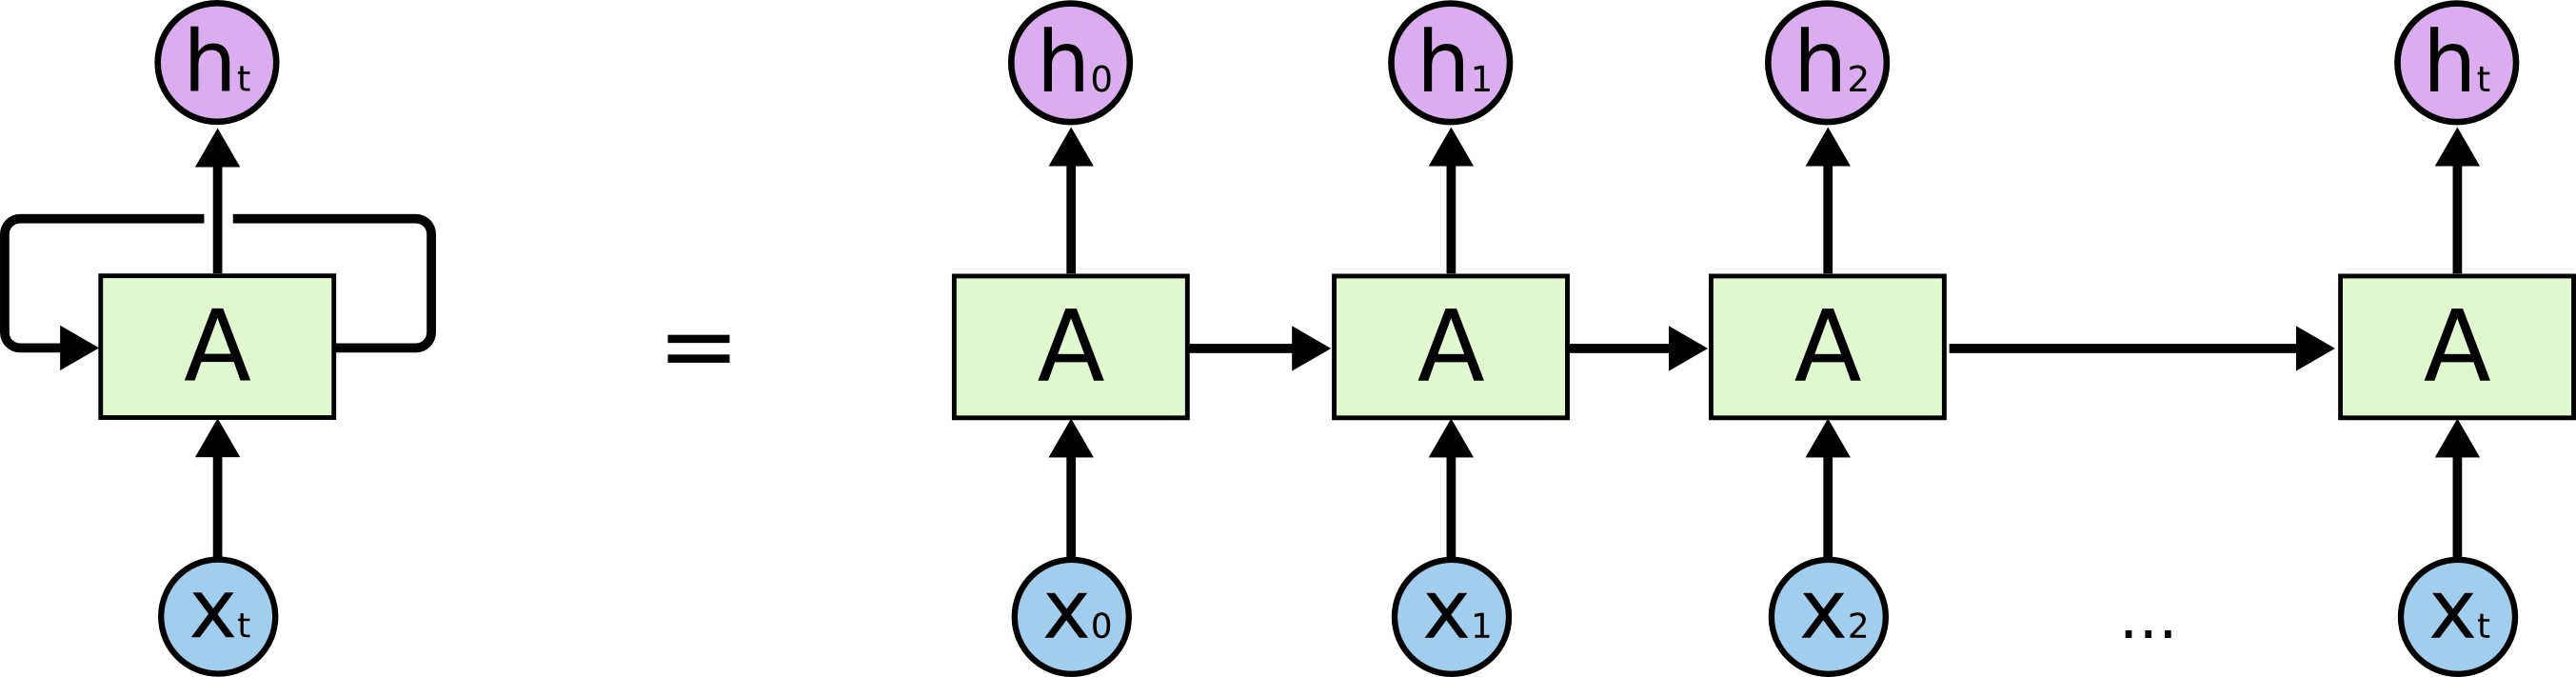
\includegraphics[scale=.4]{img/rnn.png}
		\caption{\textit{Unrolling} di una rete neurale ricorsiva}
		\label{fig:unroll}
	\end{figure*}
	Nella Figura \ref{fig:unroll} si può vedere come, preso un ciclo, una \texttt{RNN} si può interpretare come una successione di copie della stessa rete. La loro struttura \textit{a catena} si adatta perfettamente al processamento di sequenze e liste. L'interpretazione è la seguente: data un porzione di rete $A$, essa guarda l'input $x_t$ e produce l'output $h_t$, permettendo tramite il loop di passare l'informazione dal passo $t$ a $t + 1$. Una \texttt{RNN} può quindi guardare dietro nel tempo, individuare una dipendenza fra passato e presente e quindi produrre l'output più opportuno. La domanda ora è la seguente: \textit{quanto} indietro nel tempo? Sfortunatamente, le \texttt{RNN} perdono efficacia man mano che la distanza tra passato interessante e presente aumenta.
	
	\subsection{Long Short Term Memory}
		Le \textit{Long Short Term Memory} (\texttt{LSTM}) sono un particolare tipo di \texttt{RNN} capaci di apprendere dipendenze a lungo termine. Infatti, le \texttt{LSTM} sono state proposte proprio per ovviare al problema delle \texttt{RNN} precedentemente descritto. I moduli, in questo tipo di architettura (Figura \ref{fig:lstm}), racchiudono al loro interno più layer con funzione di attivazione \texttt{sigmoid} e \texttt{tanh} che interagiscono fra loro in maniera ben specifica.
		
		\begin{figure*}[h]
			\centering
			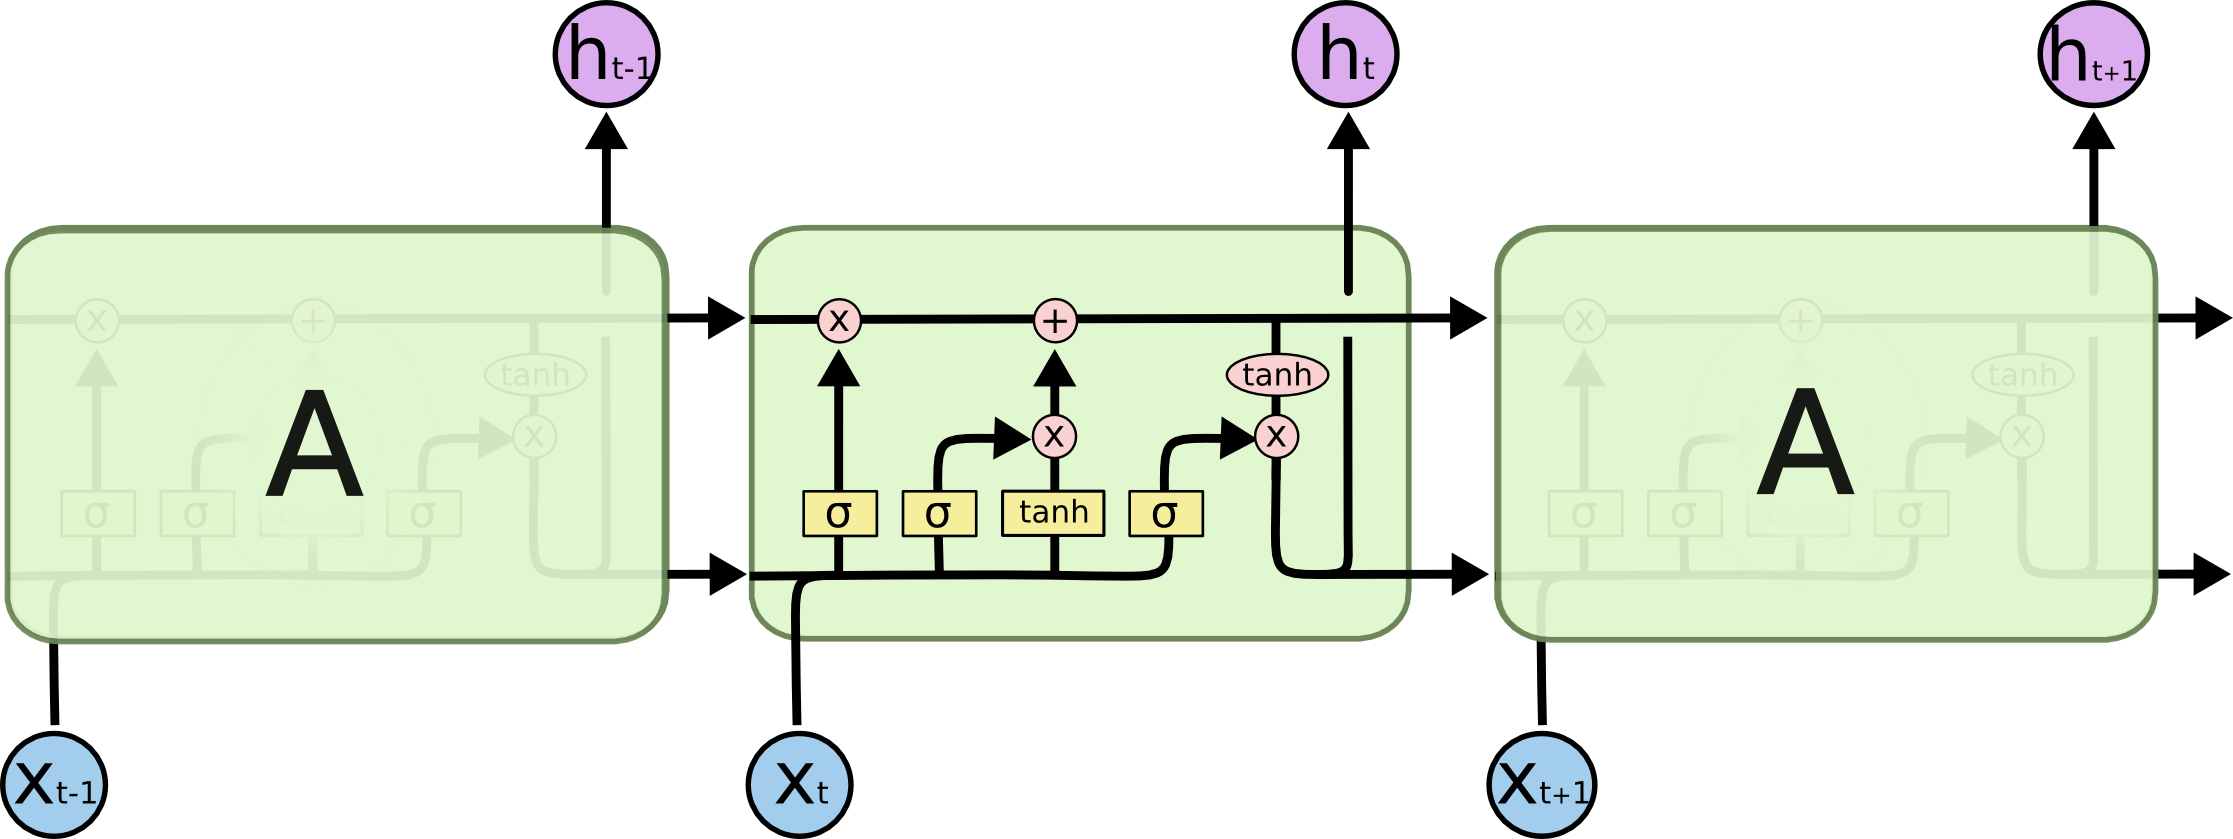
\includegraphics[scale=.5]{img/lstm.png}
			\caption{Esempio di struttura interna alla base delle \textit{Long Short Term Memory (\texttt{LSTM})}}
			\label{fig:lstm}
		\end{figure*}
	
		L'idea alla base è che la \texttt{LSTM} può rimuovere o aggiungere informazioni allo stato della sua cella. Tali scelte vengono influenzate da strutture chiamate \textit{porta} (o \textit{gate}). Una porta fa passare l'informazione nello stato della cella in maniera ottimale, dato che la porta stessa non è altro che uno strato di rete neurale con funzione di attivazione sigmoidea (cella $\sigma$ in Figura \ref{fig:lstm}). Si ricordi che il range di $\sigma$ è compreso fra $0$ (\textit{non far entrare nulla}) e $1$ (\textit{fai entrare tutto}). Seguono ora brevemente i passi che ci sono dietro al funzionamento di una \texttt{LSTM}.
		
		\paragraph{Informazioni da dimenticare}
			All'arrivo dell'input $x_t$, la prima cosa da fare è decidere quale informazione precedentemente ottenuta va buttata via. Viene prelevato l'output $h_{t - 1}$ e l'input attuale $x_t$, e restituito il valore compreso fra $0$ e $1$ per ogni numero nello stato della cella $C_{t - 1}$.
		
		\paragraph{Nuove informazioni e aggiornamento dello stato}
			Il prossimo passo è quello di decidere quali informazioni assorbire nello stato della cella. Uno strato con attivazione \texttt{tanh} crea un vettore di valori candidati che potrebbero essere aggiunti al futuro $C_t$.
		
		\paragraph{Output}
			

		\begin{itemize}
			\item rnn
			\item dipendenze a lungo termine
			\item lstm, l'idea che c'è dietro
			\item guida passo per passo
			\item blstm
		\end{itemize}

\section{Costruzione del Modello}\label{sec:building}

1. spiegazione formale metriche

2. quali risultati sono stati raggiunti su questo corpus

Esiste una moltitudine di approcci per individuare i fenomeni prosidici nel parlato. Restringendo la visione al solo campo del \textit{Machine Learning}, sono stati proposti in passato metodi supervisionati (vedere \cite[Capitolo 4]{bib:fenomeni-prosodici-prominenza}).

\begin{verbatim}

// LSTM_17
Overall scores:
Accuracy 90.83%
Precision 86.35%
Recall 86.08%
F1: 86.22%

// LSTM_32
Overall scores:
Accuracy 90.88%
Precision 86.38%
Recall 86.24%
F1: 86.31%

// BLSTM_17x2
Overall scores:
Accuracy 91.39%
Precision 87.11%
Recall 87.04%
F1: 87.07%
\end{verbatim}

\newpage\null\pagestyle{empty}\newpage
\newpage\null\pagestyle{empty}\newpage
\newpage\null\pagestyle{empty}\newpage

\section{Corpus PROVVISORIO}
	Nel file coi dati si ha che:
	\begin{itemize}
		\item i dati di ogni sillaba per ogni enunciato formano un unico blocco separato da una riga vuota;
		\item i dati di ogni sillaba contengono 15 feature in 3 blocchi (1 blocco per la sillaba precedente, la corrente e la successiva), sono 5 feature:
		\begin{enumerate}
			\item durata nucleo;
			\item spectral emphasis;
			\item loudness;
			\item tilt;
			\item durata sillaba.
		\end{enumerate}
	\end{itemize}
	Quindi sarà necessario scartare il primo e l'ultimo blocco (le LSTM analizzano la 
	sequenza da sole e quindi non hanno bisogno del prima e del dopo) e mantenere per ogni sillaba solo i 5 dati centrali. L'ultima colonna (0/1) indica la prominenza o meno etichettata manualmente.
	
	Dovrebbero esserci 120 enunciati. Per riprodurre gli esperimenti del paper \cite{bib:prominence-detection-italian} andranno divisi in 85/train, 15/validation e 20/test, campionandoli casualmente e ripetendo la procedura di campionamento/training/valutazione risultati per 20 volte e mediando le performance finali.
	
\section{Costruzione LSTM}
	\begin{verbatim}
		____________________________________________________________________________________________________
		Layer (type)                     Output Shape          Param #     Connected to                     
		====================================================================================================
		bidirectional_20 (Bidirectional) (None, 34, 34)        3128        bidirectional_input_20[0][0]     
		____________________________________________________________________________________________________
		dropout_20 (Dropout)             (None, 34, 34)        0           bidirectional_20[0][0]           
		____________________________________________________________________________________________________
		timedistributed_20 (TimeDistribu (None, 34, 3)         105         dropout_20[0][0]                 
		====================================================================================================
	\end{verbatim}
	
	\begin{itemize}
		\item in keras va implementato un modello sequence to sequence;
		\item in input ci va una matrice (5, 34), il padding consiste di vettori nulli di lunghezza 5;
		\begin{itemize}
			\item[\textbf{\checkmark}] padding fatto con Keras
		\end{itemize}
		\item \textbf{mi trovo a questo punto}
		\begin{itemize}
			\item[\textbf{?}] la forma dei dati va bene o serve un embedded layer?
		\end{itemize}
		\item a questo punto, come definisco l'architettura della rete
		\begin{itemize}
			\item[\textbf{?}] quanti layer ci devono essere e di che tipo?
			\item[\checkmark] provato un modello con 86\% di accuratezza
			\item provare sequence2sequence
			\item provare a implementare lavori dalla discussione (leggere domani)
			\item dopo aver provato l'inserzione di Timedistributed informarsi anche su Bidirectional
		\end{itemize}
	\end{itemize}
	Durante la costruzione, in futuro, provare a vedere come si comporta la rete in modalità \texttt{stateful = True} e al contrario.

\section{Lettura \cite{bib:fenomeni-prosodici-prominenza}}
	\subsection{Rassegna termini e metodi}
		\begin{itemize}
			\item definizione formale di prominenza;
			\item \textit{stress} e \textit{intonazione} (\textbf{pitch}, oppure \textbf{tono}) principali attori di collegamento fra prominenza e informazioni fonetico acustiche negli ennunciati;
			\item secondo alcuni studi il \textit{profilo del pitch} (variazione della frequenza fondamentale) risulta essere il più importante indicatore, poi lunghezza e infine intensità;
			\item teoria \textbf{pitch accent} [1958], proposta per stabilire equivalenza netta tra prominenza e fenomeni collegati all'intonazione e quindi alla configurazione assunte dalla frequenza fondamentale; però questo teoria è una presa di posizione troppo netta;
			\item teoria \textbf{metrica} [1975], creazione di albero metrico e griglia metrica, infine creazione della strutture \textit{tune};
			\item \textbf{isocronia} [1979], la prominenza è un fenomeno ritmico che avviene a intervalli di tempo regolari, ma lo studio viene messo in dubbio da alcuni test empirici;
			\item \textit{tone languages} (cinese mandarino) e \textit{stress languages} (inglese), nella prima categoria il pitch determina anche il significato della parola: poi però c'è una via di mezzo che sono le \textit{pitch-accented langauges};
			\item \textit{stress lessica} e \textit{stress frasale};
			\item verranno trattate lingue stress accented (inglese, spagnolo, olandese, italiano...);
			\item vengono individuati essenzialmente due attori principali nella definizione di prominenza:
			\begin{itemize}
				\item pitch accent
				\item stress (frasale)
			\end{itemize}
		\end{itemize}
	
	\subsection{Analisi fonetico-acustica}
		\begin{itemize}
			\item tre misure:
			\begin{itemize}
				\item segmentazione ennunciato e misure di durata, lo studio si baserà su unità di tipo sillabico; è necessario identificare nuclei sillabici dato che hanno le stesse caratteristiche delle sillabe intere, ma queste ultime sono difficili da identificare nel parlato; algoritmo:
					\begin{enumerate}
						\item isolamento dei nuclei
						\item identificazione dei confini dei nuclei
						\item durata dei nuclei sillabici
					\end{enumerate}
				\item misure relative ai profili intonativi (\textbf{\textit{pitch}}); i suoni \textbf{sonori} sono prodotti esclusivamente dalle corde vocali e poi ci sono quelli \textbf{sordi}. La frequenza fondamentale risulta nulla durante qualli sordi quindi il profilo del pitch risulterà definito esclusivamente in corrispondenza dei suoni sonori;
				\item misure relative all'intensità o energia;
			\end{itemize}
		\end{itemize}
	
	\subsection{Identificazione dei fenomeni prosodici}
		\begin{itemize}
			\item ricordiamo: per riconoscere fenomeno prosodico c'è bisogno dello stress della sillaba (fenomeno a carico del nucleo sillabico), o la presenza di un pitch accent all'interno della sillaba analizzata;
			
		\begin{figure*}
			\begin{table}[H]
				\label{my-label}
				\begin{tabular}{l|c|c|c|c}
					Fenomeni percettivi & \multicolumn{4}{c}{Prominenza}                                                                                                                                                               \\ \hline
					Fenomeni prosodici  & \multicolumn{2}{c}{Stress}                                         & \multicolumn{2}{c}{Pitch accent}                                                                                       \\ 
					Fenomeni acustici   & durata & \begin{tabular}[c]{@{}c@{}}enfasi\\ spettrale\end{tabular} & \begin{tabular}[c]{@{}c@{}}movimenti\\ in F0\end{tabular} & \begin{tabular}[c]{@{}c@{}}intensità\\ globale\end{tabular}
				\end{tabular}
			\end{table}
		\end{figure*}
		\end{itemize}
	
\section{Lettura \cite{bib:prominence-by-acoustic-analyses}}
	\begin{itemize}
		\item come è possibile definire la prominenza?
		\item qual è il miglior dominio di promineneza in acustica? sillabi;
		\item la prominenza è un fenomeno discreto o continuo? fenomeno continuo o multilivello;
		\item quali sono i parametri che combinati spiegano la prominenza? 
		\item ci sono parametri universali inter-linguistici?
		\item meglio gli approcci rulebase o machine learning?
		\item come possono essere valutati correttamente i sistemi di valutazione automatica?
	\end{itemize}

	Si può dare una prima parziale formalizzazione della prominenza:
	\begin{equation}
		\label{eq:prom}
		Prom^i = FA^i + PA^i
	\end{equation}
	$FA$ indica l'accento di forza, mentre $PA$ il pitch accent, il tutto all'$i$-esimo segmento.

\section{Lettura \cite{bib:prominence-detection-italian}}
	Vengono usate le (a partire da CRF che captano solo funzioni lineari) CNF, LDCRF, e le LDCNF. Questi tipi di PGM (Probabilistic Graphical Model) sono in grado di maneggiare sequenze di input output facendo previsioni su quella di output, considerando le configurazioni d input.
	\begin{itemize}
		\item l'$i$-esimo nodo in input prende un vettore di features;
		\item l'$i$-esimo nodo in output assegna un label, condizionato dai relativi vettori di features in input.
	\end{itemize}

	Vengono spiegati i vari tipi di \texttt{PGM} e il modo in cui è stato creato il corpus. Risultati ottenuti.

\section{Concetti Base}
	\subsection{Reti Deep: LSTM}
		Come descritto in \cite{bib:prominence-by-acoustic-analyses}, i principali vantaggi di usare metodi machine learning sono:
		\begin{itemize}
			\item approccio induttivo, il modello è appreso dai dati;
			\item classificazione rapida;
			\item rilevatori/classificatori altamente precisi.
		\end{itemize}
		Gli svantaggi invece consistono in:
		\begin{itemize}
			\item necessità di grossi corpora annotati per apprendere;
			\item i sistemi rischiano di essere legati allo specifico corpora o alla lingua usata durante la fase di apprendimento;
			\item i modelli prodotti sono tipicamente \textit{a scatola chiusa}, non c'è modo di estrarre informazioni linguistiche utili.
		\end{itemize}
		
\begin{thebibliography}{99}	
	\bibitem{bib:fenomeni-prosodici-prominenza}
		Fabio Tamburini,
		\newblock \emph{Fenomeni Prosodici e Prominenza: Un Approccio Acustico},
		2005.
	
	\bibitem{bib:prominence-detection-italian}
		Fabio Tamburini, Chiara Bertini, Pier Marco Bertinetto,
		\newblock \emph{Prosodic prominence detection in Italian continuous speech using probabilistic graphical models},
		2014
		
	\bibitem{bib:prominence-by-acoustic-analyses}
		Fabio Tamburini,
		\newblock \emph{Automatic Detection of Prosodic Prominence by Means of Acoustic Analyses},
		2015
\end{thebibliography}

\end{document}
